\section{Fat-Tailed Variational Inference}

\subsection{Introduction}

\begin{frame}
    \frametitle{Variational inference}
    
    \textbf{Goal}: Given access to a proportional $\bar\pi \propto \pi$, approximate $\pi \approx q$
    
    \pause
    
    \textbf{Example}: Bayesian inference, $\pi(\theta) = p(\theta \mid x)$ and $\bar\pi(\theta) = p(x, \theta)$ 
    
    \pause
    
    \textbf{Variational inference}: $\max_{q \in \mathcal{Q}} \text{ELBO}(q, \bar\pi)$ where
    \begin{align*}
      -\text{KL}(q, \pi)
      \propto 
      \text{ELBO}(q,\bar\pi)
      &= \int q(x) \log \frac{\bar\pi(x)}{q(x)} dx\\
      & \approx \frac{1}{n} \sum_{i=1}^n \log \frac{\bar\pi(x_i)}{q(x_i)},\;
      x_i \simiid q
    \end{align*}
    \pause
    More expressive variational family $\mathcal{Q} \Rightarrow$ better approximation quality
\end{frame}

\begin{frame}{Expressive variational families using flows}
    Let $f_\theta$ be an invertible flow and $p_X(x)$ a probability density (the \emph{base distribution}).
    Consider variational family $\mathcal{Q} = \{q_\theta : \theta \in \Theta\}$ where
    \begin{align}
        \label{eq:change-of-variable}
        q_\theta(y)
          = p_{X}(f_\theta^{-1}(y)) \left\lvert \det
            \left.\frac{d f_\theta^{-1}(z)}{dz} \right\vert_{z=y}
          \right\rvert .
    \end{align}
    
    \begin{figure}
        \centering
        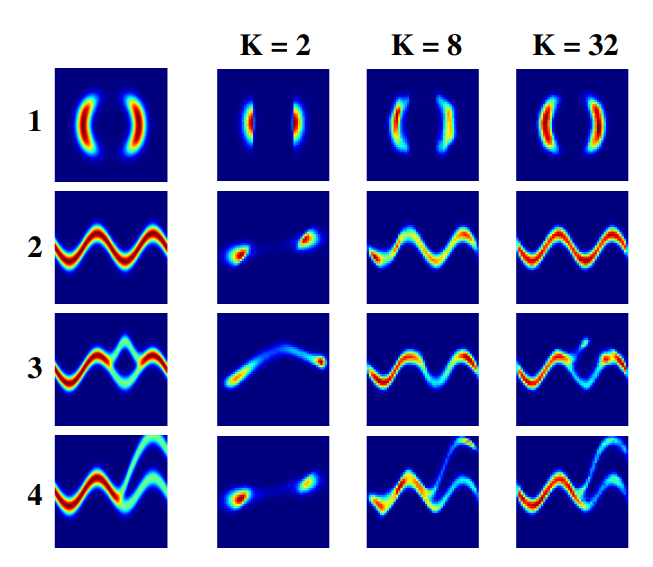
\includegraphics[width=0.3\textwidth]{Figures/ftvi/norm_flow_eg.png}
        \caption{\parencite{rezende2015variational} flows can transform a Gaussian into complex pushforward distributions}
    \end{figure}
\end{frame}

\begin{frame}
    \frametitle{Fat-tailed variational inference\footnote{\tiny \fullcite{liang2022fat}}}
    
    %%MM%% \textbf{Research aims (\cite{jaini2020tails}, this work)}: 
    %%MM%% What happens when $\pi$ is fat-tailed? What about when $\pi$ is multivariate?
    \textbf{Our Research Aims}:
    \begin{itemize}
        \item 
        What happens when $\pi$ is fat-tailed?
        \item 
        What about when $\pi$ is multivariate?
    \end{itemize}
    
    
    \begin{figure}[htbp]
      \centering
      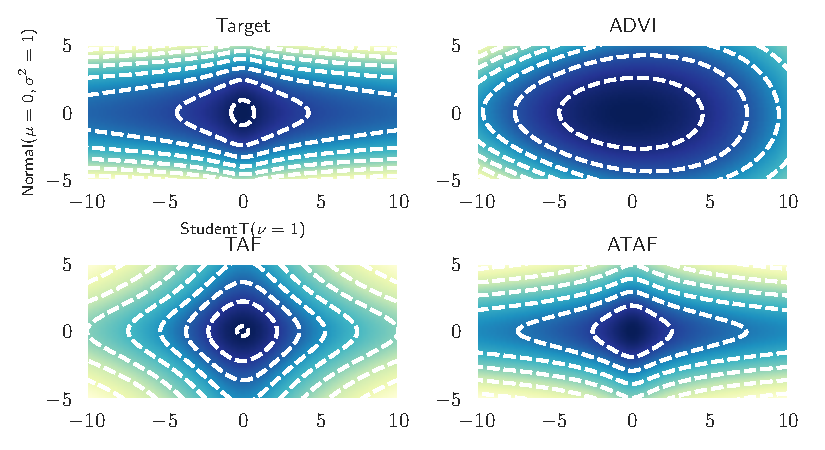
\includegraphics[width=0.7\textwidth]{Figures/ftvi/pancake.pdf}
      \label{fig:pancake}
    \end{figure}
\end{frame}

\begin{frame}{Methods}
    \textbf{Automatic Differentiation Variational Inference (ADVI, \cite{kucukelbir2017automatic,webb2019improving})}:
    
      \quad 
      $\cQ_\text{ADVI}~\coloneqq~\{
        (f_\theta)_\ast \mu
        \}$, 
      where $\mu = \text{Normal}(0_d, I_d)$.
      \vspace{3mm}
    \pause
    \textbf{Tail Adaptive Flows (TAF, \cite{jaini2020tails})}:
    
      \quad 
      $\cQ_\text{TAF}
        \coloneqq \{
        (f_\theta)_\ast \mu_\nu
        \}$,
      where $\mu_\nu = \prod_{i=1}^d \text{StudentT}(\nu)$ with $\nu \in \RR_+$.
      \vspace{3mm}
    \pause
    \textbf{Anisotropic Tail-Adaptive Flows (ATAF, this work)}:
    
      \quad 
      $\cQ_\text{ATAF}~\coloneqq~\{
        (f_\theta)_\ast \mu_{\vec{\nu}}
        \},$
      where $\mu_{\vec{\nu}} = \prod_{i=1}^d \text{StudentT}(\nu_i)$ with $\vec{\nu} \in \RR_+^d$.
\end{frame}

\subsection{Theory}

\begin{subframe}{Fat-tailed theory}
    \begin{definition}[Classification of tails]
        \label{def:tail-classification}
        For $\alpha,p > 0$, we let 
        \vspace{-1mm}
        \begin{itemize}
            \item $\mathcal{E}_\alpha^p$ denote the set of \emph{exponential-type} random variables $X$ with $\mathbb{P}(|X| \geq x) = \Theta(e^{-\alpha x^p})$ (e.g.
            $\overline{\cE_\alpha^2}$ are $\alpha^{-1/2}$-sub-Gaussians, $\overline{\cE_\alpha^1}$ are sub-exponentials).
        \vspace{-1mm}
            \item $\mathcal{L}_\alpha^p$ denote the set of \emph{logarithmic-type} random variables $X$ with $\mathbb{P}(|X| \geq x) = \Theta(e^{-\alpha(\log x)^p})$ (e.g.
            $\cL^1_\alpha$ are power laws)
        \end{itemize}
        \vspace{-1mm}
        Define the ascending families
        $\overline{\cE_\alpha^p}$ and $\overline{\cL_\alpha^p}$
        analogously as before except with $\Theta(\cdot)$ replaced
        by $\cO(\cdot)$.
    \end{definition}
\end{subframe}

\begin{frame}{Theoretical Result I}
    \begin{assumption}\label{assump:lipschitz}
        $f_\theta$ is invertible, and both $f_\theta$ and $f^{-1}_\theta$
        are $L$-Lipschitz continuous.
    \end{assumption}
    \pause
    \begin{theorem}
      \label{thm:distn_class_closed}
      \begin{itemize}[<+->]
          \item $f_\theta$ cannot make the tails of a fat-tailed distribution fatter (decrease tail parameter $\alpha$).
          \item If in addition $f_\theta$ is smooth with no critical points, then it cannot change
            the tail parameter of a fat-tailed distribution.
          \item Light-tailed distributions remain light-tailed under polynomial flows \parencite{jaini2019sum}.
      \end{itemize}
    \end{theorem}
\end{frame}

\subsubsection{Tail anisotropy}

\begin{frame}{Tail anisotropy}
    \begin{definition}[Tail anisotropy]
      \label{def:mv-tail-param}
      For random vector $X$, define
      $\alpha_X(v) = -\lim_{x \to \infty} \log \PP(\braket{v,X} \geq x) / \log x$ when the limit exists, and $\alpha_X(v) = +\infty$ otherwise.
      $X$ is \emph{tail-isotropic} if $\alpha_X(v) \equiv c < \infty$ is constant.
    \end{definition}

    \begin{figure}[htbp]
  \centering
  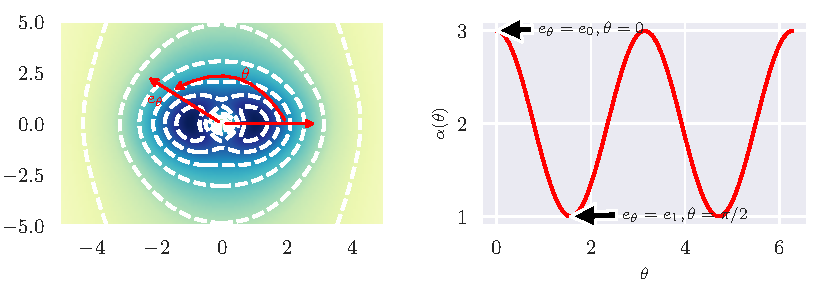
\includegraphics[width=0.85\textwidth]{Figures/ftvi/radial-fat-tail.pdf}%
%   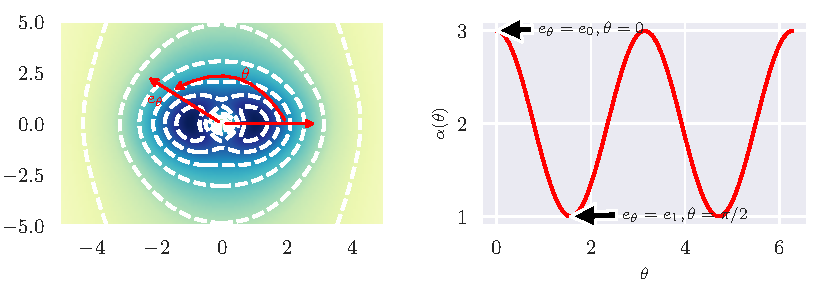
\includegraphics[trim={0 0 7cm 0},clip]{Figures/ftvi/radial-fat-tail.pdf}\\%
%   \vspace{-8mm}
%   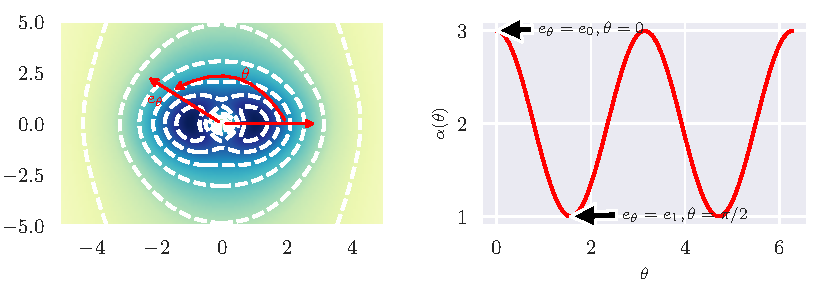
\includegraphics[trim={7.2cm 0 0 0},clip]{Figures/ftvi/radial-fat-tail.pdf}%
  %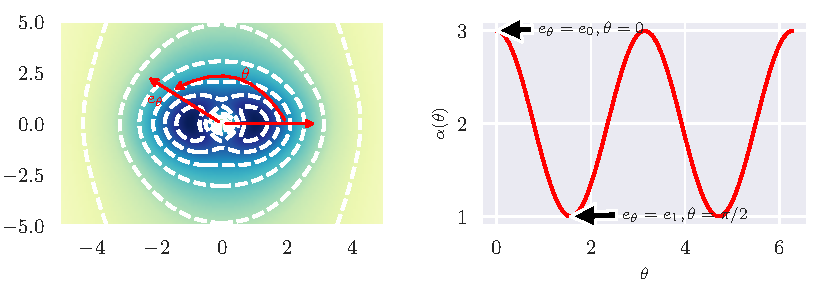
\includegraphics[width=\textwidth]{Figures/ftvi/radial-fat-tail.png}%
  %\input{Figures/ftvi/radial-fat-tail.pgf}
%   \caption{
%     A tail-anisotropic distribution with PDF $\dd P(r,\theta) = r^{-\alpha(\theta)} r \dd r \dd\theta$ (left)
%     and its tail-parameter function $\alpha(\theta) = 2 + \cos(2\theta)$ (right).
%   }
  \label{fig:radial-fat-tail}
\end{figure}
\end{frame}

% \begin{frame}{A problematic example}
%     \begin{figure}[htbp]
%     \centering
%     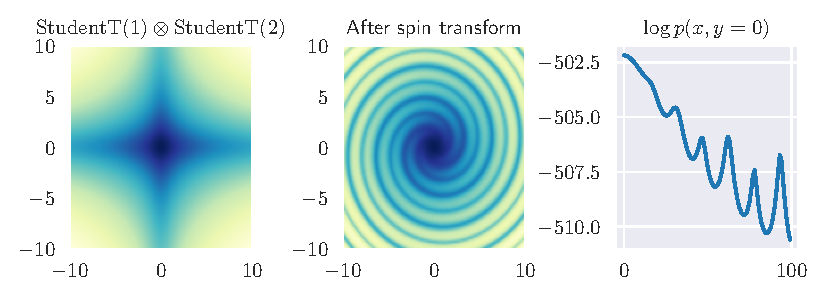
\includegraphics[width=\textwidth]{Figures/ftvi/spiral.pdf}
%     % 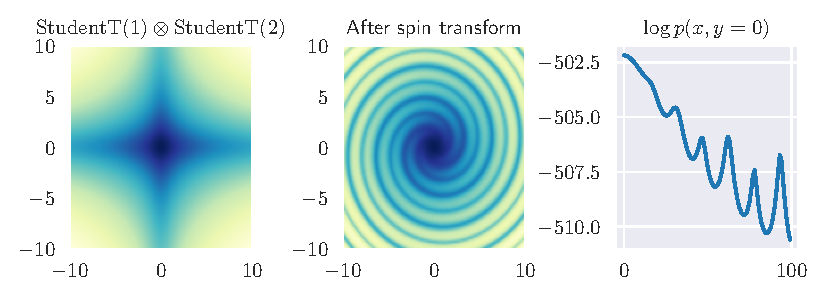
\includegraphics[trim={0 0 9cm 0},clip]{Figures/ftvi/spiral.pdf}\\
%     % 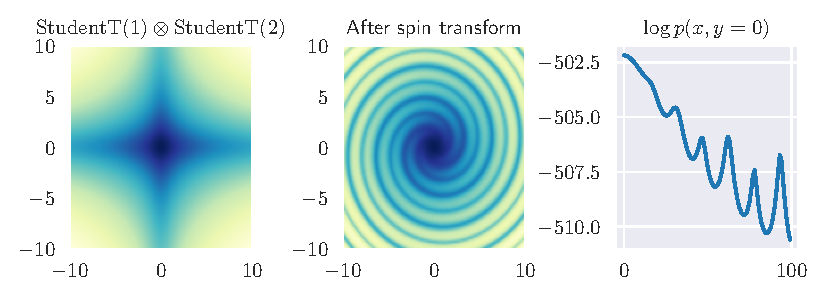
\includegraphics[trim={5cm 0 4.9cm 0},clip]{Figures/ftvi/spiral.pdf}\\
%     % 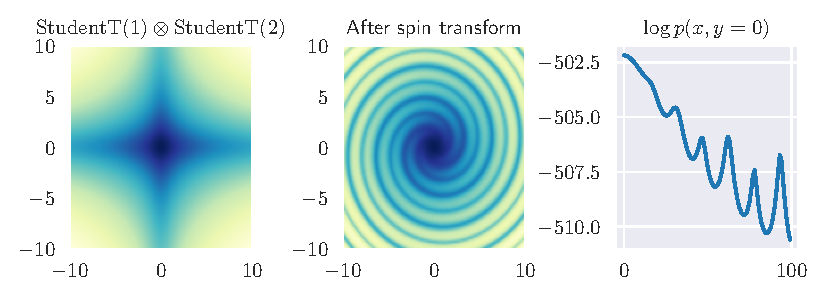
\includegraphics[trim={9.3cm 0 0cm 0},clip]{Figures/ftvi/spiral.pdf}\\

%     \label{fig:spiral}
% \end{figure}
% \end{frame}

\begin{frame}{Theoretical Result II}
    \begin{proposition}[Pushforwards of tail-isotropic distributions]
      \label{prop:isotropic-pushforward}
      Let $\mu$ be tail isotropic with non-integer parameter $\nu$
      and suppose $f_\theta$ satisfies \Cref{assump:lipschitz}.
      Then $(f_\theta)_\ast \mu$ is tail isotropic with parameter $\nu$.
    \end{proposition}
    
    \therefore\quad ATAF is necessary for anisotropic tails

    % \begin{remark}\label{remark:anisotropic}
    %   ATAF can represent tail-anisotropic distributions with up to $d$ different
    %   tail parameters while simultaneously satisfying \Cref{assump:lipschitz}.
    %   For example, if $\Phi_\text{Flow} = \text{Identity}$ and $\mu_\nu = \prod_{i=1}^d \text{StudentT}(i)$
    %   then the pushforward $(\Phi_\text{Flow})_\ast \mu_\nu = \mu_\nu$ is tail-anisotropic.
    %   % Moreover, its standard basis tail parameters are equal
    %   % (up to permutation) to those for $\mu$.
    % \end{remark}
\end{frame}

\subsection{Experiments}

\begin{subframe}{Bayesian linear regression}
\vspace{-10mm}
    \begin{gather*}
        \sigma^2 \sim \text{Inv-Gamma}(a_0, b_0)\\
        \beta \mid \sigma^2 \sim \cN(0, \sigma^2),\qquad
        y \mid X, \beta, \sigma \sim \cN(X \beta, \sigma^2) ,
    \end{gather*}
    
    The posterior is tail-anisotropic: 
    
    $p(\sigma^2, \beta=c \mid X, y) \propto \rho(\sigma^2) \in \cL^1_{\alpha_n}$ is fat-tailed (power-law)
    
    $p(\sigma^2=c, \beta \mid X, y) \propto \rho(\beta \mid c) \in \overline{\cE^2}$ is light-tailed (sub-Gaussian)

    % The posterior is tail-anisotropic since $p(\beta,\sigma^2 \mid X, y) = \rho(\sigma^2)\rho(\beta \mid \sigma)$ where $\rho(\beta \mid \sigma) = \cN(\Sigma_n(X^\top X \hat\beta), \sigma^2 \Sigma_n)$, $\Sigma_n = (X^\top X + \sigma^{-2})^{-1}$, $\hat\beta = (X^\top X)^{-1} X^\top y$, and
    % %\begin{align*}
    %     %p(\beta,\sigma^2 \mid X, y) &= \rho(\sigma^2) \rho(\beta \mid \sigma) \\
    %     \[
    %     \rho(\sigma^2) = \text{Inv-Gamma}\bigg(
    %     %\underbrace{a_0 + \frac{n}{2}}_{\eqqcolon a_n}, 
    %     a_0 + \frac{n}{2}, 
    %     b_0 + \frac{1}{2}(y^\top y - \mu_n^\top \Sigma_n \mu_n)\bigg). % \\
    %     \]
    %     %\rho(\beta \mid \sigma) &= \cN(\Sigma_n(X^\top X \hat\beta), \sigma^2 (X^\top X + \sigma^{-2} I)^{-1})
    % %\end{align*}
    % So for fixed $c$ we have that $p(\sigma^2, \beta=c \mid X, y) \propto \rho(\sigma^2) \in \cL^1_{\alpha_n}$
    % as a function of $\sigma$
    % and $p(\sigma^2=c, \beta \mid X, y) \propto \rho(\beta \mid c) \in \overline{\cE^2}$
    % as a function of $\beta$.
\end{subframe}

\begin{subframe}
    \begin{figure}[htbp]
  \centering
  \vspace{-0.2cm}
  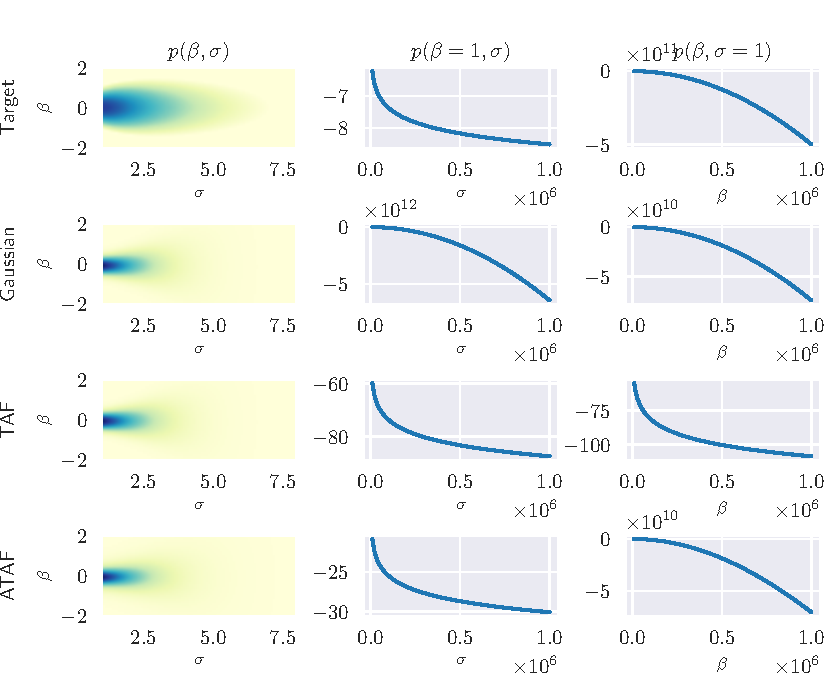
\includegraphics[width=0.75\textwidth]{Figures/ftvi/blr_aniso.pdf}
  \vspace{-0.3cm}
%   \caption{
%     Bayesian linear regression's tail-anisotropic posterior
%     (top left) exhibits a fat-tailed conditional in $\sigma$ (as evidenced by
%     the convex power-law decay in the top middle panel) and a Gaussian conditional in $\beta$ (concave graph in top right panel).
%     While all methods appear to provide a good approximation of the bulk (left column),
%     \Cref{prop:isotropic-pushforward} implies
%     Gaussian (Gaussian, second row) or isotropic StudentT product (TAF, third row) base distributions
%     yield Gaussian or power-law tails, respectively, for \emph{both} $\sigma$ and $\beta$.
%     In contrast, ATAF (bottom row) illustrates \Cref{remark:anisotropic} by
%     modeling simultaneously a power-law tail on $\sigma$ and Gaussian tail on $\beta$.
%   }
  \label{fig:blr-anisotropic}
\end{figure}
\end{subframe}


% \begin{subframe}{diamonds \cite{ghposteriordb}}
%     \begin{gather*}
%         \alpha \sim \text{StudentT}(\nu=3, \text{loc}=8, \text{scale}=10)\\
%         \sigma \sim \text{HalfStudentT}(\nu=3, \text{loc}=0, \text{scale}=10)\\
%         \beta \sim \cN(0, \mI_{24}),\qquad
%         y \sim \cN(\alpha + X \beta, \sigma) .
%     \end{gather*}

%     \begin{table}[htbp]
%         \centering
%         \begin{tabular}{rcc}
%             \tableheadrow
%                       & \tableheadcol{ELBO}                & \tableheadcol{$\log p(y)$}       \\
%             ADVI      & $\mathbf{2873.90} \pm 6.95$    & $2969.73 \pm 1.73$ \\
%             TAF       & $2839.64 \pm 9.10$    & $2973.85 \pm 0.87$ \\
%             ATAF      & $2842.75 \pm 8.83$    & $\mathbf{2976.75} \pm 0.66$ \\
%             \hline
%             NUTS      & n/a                  & $3724.59 \pm 0.036$ \\
%         \end{tabular}
%         %\caption{diamonds}
%         \label{tab:diamonds}
%     \end{table}
% \end{subframe}

\begin{frame}{Eight schools \parencite{rubin1981estimation}}
    \begin{gather*}
        \tau \sim \text{HalfCauchy}(\text{loc}=0, \text{scale}=5)\\
        \mu \sim \cN(0, 5),\qquad
        \theta \sim \cN(\mu, \tau),\qquad
        y \sim \cN(\theta, \sigma) .
    \end{gather*}

    \begin{table}[htbp]
        \centering
        \begin{tabular}{rcc}
            \toprule
                      & ELBO                & $\log p(y)$       \\
            \midrule
            ADVI      & $-72.13 \pm 6.89$    & $-53.25 \pm 3.44$ \\
            TAF       & $-64.64 \pm 4.88$    & $-52.51 \pm 4.41$ \\
            ATAF      & $\mathbf{-58.63} \pm 4.75$    & $\mathbf{-51.01} \pm 3.71$ \\
            \hline
            NUTS      & n/a                  & $-47.78 \pm 0.093$ \\\bottomrule
        \end{tabular}
        %\caption{Eight schools}
        \label{tab:eight_schools}
    \end{table}
\end{frame}

\begin{frame}{Financial \parencite{fama2015five} and actuarial \parencite{cms} density modeling}
    \begin{table}[htbp]
    \centering
    \begin{tabular}{rcc}
        \toprule
                  & Fama-French 5 Industry Daily & CMS 2008-2010 DE-SynPUF       \\
        \midrule
        ADVI      & $-5.018 \pm 0.056$    & $-1.883 \pm 0.012$ \\
        TAF       & $-4.703 \pm 0.023$    & $-1.659 \pm 0.004$ \\
        ATAF      & $\mathbf{-4.699} \pm 0.024$    & $\mathbf{-1.603} \pm 0.034$ \\\bottomrule
    \end{tabular}
    \vspace{-2mm}
    \caption{
        Log-likelihoods (higher is better, $\pm$ standard errors).
    }
    \label{tab:density-estimation}
\end{table}
\end{frame}

% \subsection{Conclusion}

% \begin{frame}{Conclusions}
%     \begin{itemize}[<+->]
%         \item Tails of flow-based variational approximations are limited by choice of base distribution!
%         \item 
%         %%MM%% Prior work (TAF, \cite{jaini2020tails}) considers univariate tails, and in this work:
%         We improved prior work (TAF, \cite{jaini2020tails}), which considered univariate tails, in the following ways:
%         \begin{itemize}
%             \item 
%             Prior univariate theory is refined to include $\alpha$ and
%             closure results are sharpened
%             \item 
%             A multivariate theory is proposed to quantify tail-anisotropy and prove
%             ATAF's necessity
%             \item 
%             Experiments confirm ATAF's improvements on real-world fat-tailed datasets
%         \end{itemize}
%     \end{itemize}
% \end{frame}